\chapter{Pollard-rho para resolver ECDLP} \label{PR}
Em 1978, Pollard sugeriu o método Monte-Carlo\footnote{Monte-Carlo é um método estatístico que se baseiam em amostragens aleatórias massivas para obter resultados numéricos, isto é, repetindo sucessivas simulações um elevado número de vezes, para calcular probabilidades de forma heurística.} para resolver o problema do logaritmo discreto. Desde então, o método foi modificado para resolver o ECDLP. Como o algoritmo Pollard-rho é atualmente o algoritmo mais rápido para resolver o ECDLP, então a segurança do ECC depende da eficiência desse algoritmo. Teoricamente, se o algoritmo Pollard-rho é capaz de resolver o ECDLP eficientemente e em um tempo relativamente curto, então o criptossistema estará inseguro. \cite{Mandy:2007}

A estratégia do algoritmo é produzir uma sequência de termos gerados aleatoriamente $(c_k, d_k, R_k)$, em que \(R_k\) é um ponto na curva \(E\) e \(c_k\)  e \(d_k\) estão em $\mathbb{F}_p$ sobre a qual a curva elíptica \(E\) está definida. Como $E(\mathbb{F}_p)$ é um grupo finito, a sequência eventualmente irá se tornar periódica e voltará para um termo anterior da sequência \--- tal ocorrência é chamada de \textit{colisão}. Pelo paradoxo do aniversário
\footnote{Suponha que uma urna tenha \(n\) bolas numeradas de 1 a \(n\). As bolas são aleatoriamente retiradas uma de cada vez e colocadas de volta na urna. Portanto, o número esperado para que as bolas se repitam é de aproximadamente de $\sqrt{\pi n/2}$. Se \(n\) = 365 e as bolas representam diferentes dias do ano, então pode-se dizer que o número esperado de pessoas que tem de ser reunidas em uma sala para que pelo menos duas delas tenham nascido no mesmo dia é de aproximadamente $\sqrt{\pi 365/2} \approx 24$. Esse número é surpreendentemente pequeno e, consequentemente, daí vem a nomenclatura ``paradoxo do aniversário''. \cite{Guide}},
o número de iterações médio para que se obtenha uma colisão é de aproximadamente $\sqrt{\pi n/2} \approx 1.2533 \sqrt{n}$. Usa-se essa periodicidade para resolver ECDLP. Como nem sempre a sequência volta para o primeiro termo, um diagrama da sequência parecerá com a letra grega \(\rho\) (ver Figura \ref{fig:rho}). Por este motivo esse método é chamado de Pollard-rho. Essa sequência de termos gerados é chamada de ``percurso''. \cite{Guide}

Seja \(\mu\) o tamanho da cauda e \(\lambda\) o tamanho do ciclo. Após um número finito de iterações, obtêm-se os termos $R_k = R_{k+\lambda}$, em que $k > \mu$ e $\lambda > 1$. Neste ponto, já deverá ter sido encontrado uma correspondência entre os termos e poderá empregar resultados de matemática discreta para resolver os problemas de logaritmo discreto gerado pelos elementos do conjunto finito.

A seguir serão apresentados o algoritmo de Pollard-rho e suas variações.

\begin{figure}[h]
\centering
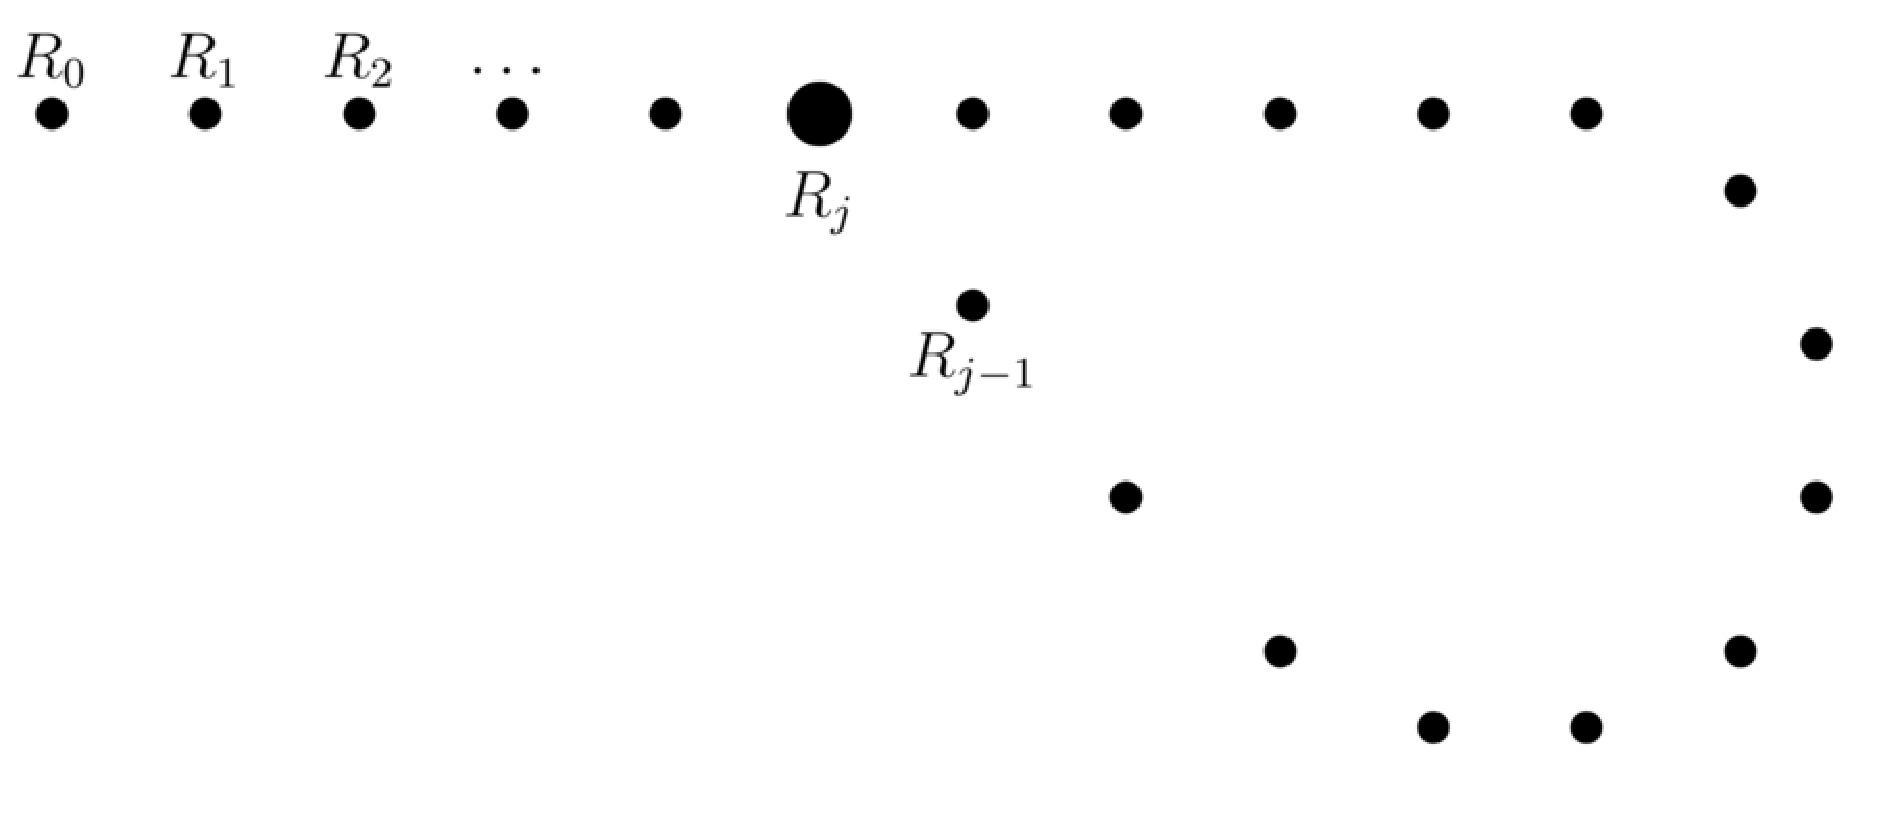
\includegraphics[scale=0.4, bb=0 0 888 376]{figuras/rho.eps}
\caption{Diagrama da sequência produzida pelo algoritmo Pollard-rho}
\label{fig:rho}
\end{figure}

\section{Pollard-rho original} \label{Pollard_original}

Uma forma simplificada de encontrar uma colisão seria selecionar inteiros aleatórios $c, d \in [0, n-1]$ e armazenar as triplas $(c, d, cP + dQ)$ em uma tabela ordenada pelo terceiro componente até que um ponto $cP + dQ$ seja obtido pela segunda vez. A desvantagem desse algoritmo é que a capacidade de armazenamento necessária para o cálculo é de $\sqrt{\pi n/2}$ triplas.

Com o algoritmo Pollard-rho, é possível encontrar os pares ($c_m, d_m$) e ($c_{2m}, d_{2m})$ aproximadamente no mesmo tempo que o algoritmo citado acima, mas tem desprezíveis requisitos de armazenamento. A ideia é definir uma função de iteração $f : \langle P \rangle \to \langle P \rangle$ de modo que $X \in \langle P \rangle$ e $a, b \in [0, n-1]$ com $X = aP + bQ$. Além disso, \(f\) deve ter características de uma função aleatória. \cite{Guide}

Seja um grupo $G = E(\mathbb{F}_p)$, tal que a ordem de $\#E(\mathbb{F}_p) = |G| = n$, e \(P\) e \(Q \in E(\mathbb{F}_p)\) tal que $Q = xP$ em \(G\). O objetivo é calcular \(x\). Segue os passos do algoritmo original proposto por Pollard:

\begin{enumerate}
\item \(G\) é particionado em 3 conjuntos $S_1, S_2, S_3$ de aproximadamente do mesmo tamanho, em que $\mathcal{O} \notin S_2$.
\item Definir uma função de iteração $f : R \to R$ de um percurso aleatório:

\begin{eqnarray} \label{eq:walk}
R_{k+1} = f(R_k) =
\begin{cases}
Q + R_k, &R_k \in S_1 \\
2R_k, &R_k \in S_2 \\
P + R_k, &R_k \in S_3
\end{cases}
\end{eqnarray}

\item Seja $R_k = c_kP + d_kQ$, e portanto

\begin{eqnarray}
c_{k+1} =
\begin{cases}
c_k, &R_k \in S_1 \\
2c_k \pmod n, &R_k \in S_2 \\
c_k + 1, &R_k \in S_3
\end{cases}
\end{eqnarray}

e

\begin{eqnarray}
d_{k+1} =
\begin{cases}
d_k + 1, &R_k \in S_1 \\
2d_k \pmod n, &R_k \in S_2 \\
d_k, &R_k \in S_3
\end{cases}
\end{eqnarray}

\item Os termos iniciais são: $R_0 = P, c_0 = 1, d_0 = 0$ e os pares gerados $(R_k, R_{2k})$ até encontrar uma correspondência $R_m = R_{2m}$, para qualquer \(m\).

\item Uma vez encontrados, calcule:

\begin{eqnarray*}
R_m = c_mP + d_mQ \\
R_{2_m} = c_{2m}P + d_{2m}Q
\end{eqnarray*}

\item Com isso, é possível calcular \(x\):

\begin{equation} \label{eq:x}
x = \frac{c_{2m} - c_m}{d_m - d_{2m}} \pmod n
\end{equation}

\end{enumerate}

O termo $(d_m - d_{2m})^{-1} \pmod n$ em (\ref{eq:x}) somente é possível calcular quando o gcd$(d_m - d_{2m}, n) = 1$, ou seja, quando \(d_m\) e \(d_{2m}\) são coprimos entre si. Caso contrário, o algoritmo retorna um valor indefinido.

%
% Pollar-rho com um processador
%
\section{Pollard-rho com único processador} \label{sec:single}

A função de iteração proposta por Pollard no algoritmo descrito na Seção \ref{Pollard_original} particionava o conjunto $G = E(\mathbb{F}_p)$ em \(L = 3\) subconjuntos \(S_1, S_2, S_3\). Alguns estudos demonstram que essa função de iteração proposta por Pollard não é suficientemente aleatória, e consequentemente, demora para encontrar uma colisão. Uma alternativa encontrada foi particionar o conjunto $G = E(\mathbb{F}_p)$ em vários subconjuntos $S_L$, por exemplo, \(L = 100\), em vez de apenas três, como fora proposto por Pollard. \cite{Laporta:2014}.

Seja $\{S_1, S_2, ..., S_L\}$ uma partição aleatória de $\langle P \rangle$ em uma quantidade \(L\) de conjuntos de aproximadamente do mesmo tamanho. Então um ponto $X \in \langle P \rangle$ pode ser designado a \(S_j\) se os cinco \textit{bits} menos significantes da coordenada \(x\) de \(X\) representam o inteiro \(j-1\). Desta forma, define-se $j = H(X)$ se $X \in S_j$, no qual \(H\) é uma função de partição. Finalmente, seja $c_j, d_j \in [0, n-1]$ para $1 \leq j \leq L$. Então $f : \langle P \rangle \to  \langle P \rangle$ é definido por

\begin{equation*}
f(X) = X + c_jP + d_jQ \textrm{, em que } j = H(X)
\end{equation*}

O pseudoalgoritmo está descrito em anexo (\ref{alg:single}).

%
% Floyd's cycle-finding
%
\subsection{Algoritmo Busca-Ciclos de Floyd} \label{floyd}
Pollard-rho é uma variante do algoritmo busca-ciclos de Floyd (\textit{Floyd's cycle-finding}), que é importante para detectar a ocorrência de um ciclo em sequências arbitrárias, seja em estruturas de dados ou geradas por sequências pseudo-aleatórias e grafos. Este algoritmo, também é chamado de algoritmo ``lebre e tartaruga'', no qual se utiliza apenas dois ponteiros que se movem através da sequência com diferentes velocidades.

Para encontrar \(R_i = R_j\), o algoritmo calcula as triplas $(c_i, d_i, R_i)$ e $(c_{2i}, d_{2i}, R_{2i})$ até que \(R_i = R_{2i}\). Para cada iteração, calcula-se \(R_{i+1} = f(R_i)\) e \(R_{2(i+1)} = f(f(R_{2i}))\), o que significa que este algoritmo utiliza uma quantidade mínima de armazenamento. O algoritmo busca-ciclos de Floyd é baseado na seguinte ideia. \cite{Ping:2011} \cite{Brent:2008}

\textbf{Teorema 1} (\cite{Knuth:1997}). Para uma sequência periódica \(\{R_0, R_1, R_2, ...\}\), existe um \(i > 0\) tal que \(R_i = R_{2i}\) e o menor valor de \(i\) que pertença ao intervalo \(\mu \leq i \leq \mu + \lambda\). \(\mu\) e \(\lambda\) são o pré-período (cauda) e o período (ciclo) da sequência \(R_i\), respectivamente.

O melhor caso desse algoritmo são necessários \(\mu\) iterações e o pior caso \(\mu + \lambda\) iterações. Sob a suposição de que \(f : G \to G\) se comporta como uma função verdadeiramente aleatória, o número esperado de iterações antes que se encontre uma colisão é de $\sqrt{\pi^5 |G|/288} \approx 1.03 \sqrt{|G|}$ \cite{Brent:2008}. O ponto chave para esse algoritmo é que precisa-se de três operações de grupo e uma comparação para cada iteração, o que o torna ineficiente.

%
% Pollard-rho com multiprocessadores
%
\section{Pollard-rho multiprocessadores} \label{sec:parallelized}
Suponha agora que \(M\) processadores estão disponíveis para resolver uma instância de ECDLP. Uma abordagem normal seria de executar o algoritmo Pollard-rho independente para cada processador (com diferentes pontos \(X_0\) aleatórios escolhidos inicialmente) até que algum dos processadores finalize. Uma análise cuidadosa mostra que o número esperado de operações de curva elíptica executadas por cada processador até que algum finalize é de $3\sqrt{n/M}$. Assim a aceleração esperada é dada pelo fator $\sqrt{M}$. \cite{Guide}

Van Oorschot e Wiener propuseram uma variante do algoritmo Pollard-rho que produz um fator de aceleração \(M\) quando \(M\) processadores são empregados. A ideia é permitir que as sequências $\{X_i\}_{i \geq 0}$ geradas pelos vários processadores possam colidir umas com as outras. Ou seja, cada processador escolhe aleatoriamente seu próprio ponto inicial \(X_0\), mas todos processadores utilizam a mesma função de iteração \(f\) para calcular os pontos subsequentes \(X_i\). Desta forma, se as sequências de dois processadores diferentes colidirem entre si, como ilustrado na Figura \ref{fig:paralellized}, as duas sequências serão idênticas daquele ponto em diante. A sequência gerada pelos processadores 3 e 4 se colidem em X. O algoritmo informa a colisão em Y, o primeiro ponto distinto subsequente \cite{Van:1996}.

\begin{figure}[h]
\centering
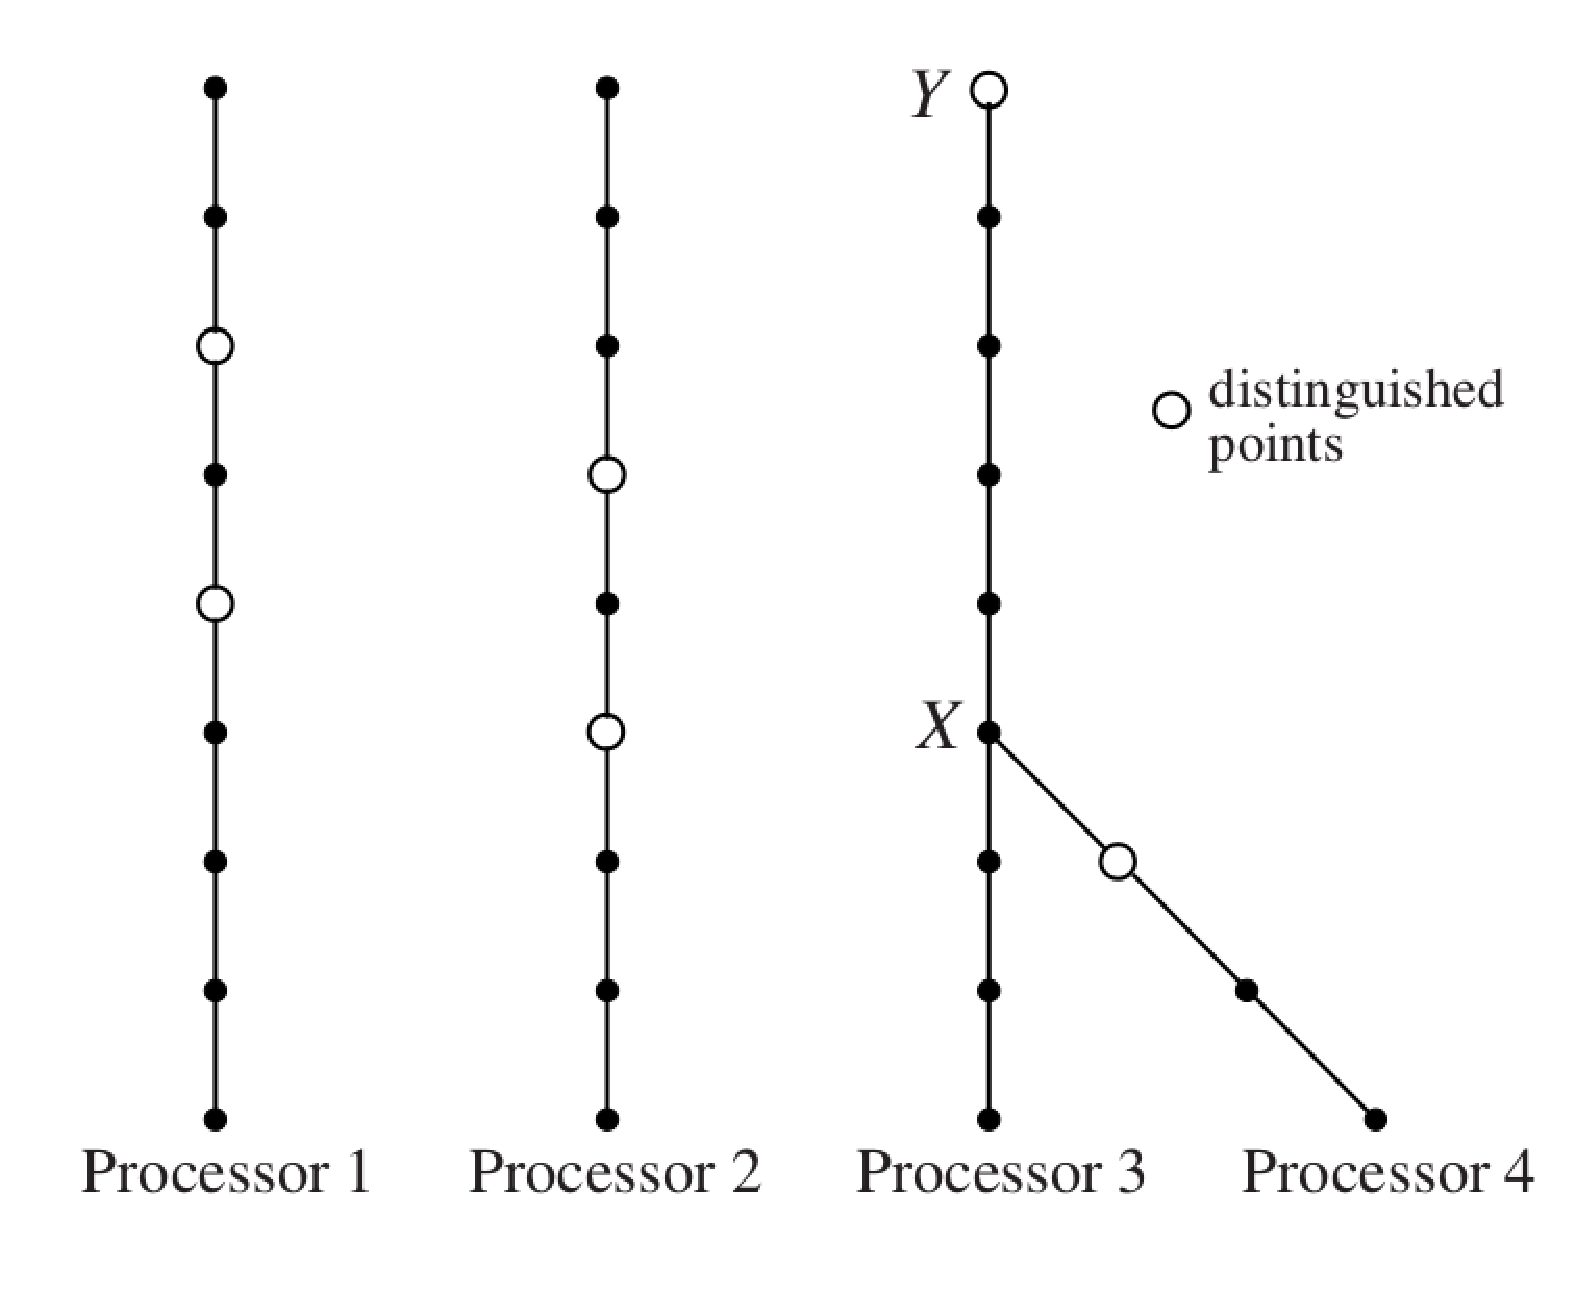
\includegraphics[scale=0.4, bb=0 0 737 604]{figuras/paralellized.eps}
\caption{A sequência gerada pelo algoritmo Pollard-rho paralelizado. }
\label{fig:paralellized}
\end{figure}

O algoritmo busca-ciclos de Floyd -- descrita na Seção \ref{floyd} -- encontra uma colisão na sequência gerada por um único processador. A seguinte estratégia possibilita uma procura eficiente de uma colisão nas sequências geradas por diferentes processadores. Uma \textit{propriedade distintiva} facilmente testável de pontos é selecionada. Por exemplo, um ponto deve ser \textit{distinto} se os primeiros \(t\) \textit{bits} de sua coordenada \(x\) são iguais a zero. Seja \(\theta\) a proporção em $\langle P \rangle$ tendo essa propriedade distintiva. Sempre que um processador encontra um ponto distinto, ele transmite o ponto a um servidor central que o armazena em uma lista ordenada. Quando o servidor recebe o mesmo ponto distinto pela segunda vez, ele calcula o logaritmo discreto desejado pela Eq. \ref{eq:x} e termina a execução de todos os processadores. O número esperado de passos por processador antes de uma colisão ocorrer é de $(\sqrt{\pi n/2})/M$. Um ponto distinto subsequente é esperado para após $1/\theta$ passos. Consequentemente o número médio (dado um número muito grande de tentativas) de operações de curva elíptica desempenhadas por cada processador antes de uma colisão de pontos distintos é de

\begin{equation}
\dfrac{1}{M} \sqrt{\dfrac{\pi n}{2}} + \dfrac{1}{\theta} \label{eq:execParallelized}
\end{equation}

A sua versão paralelizada do algoritmo Pollard-rho obtém um aumento de velocidade que é linear em relação à quantidade de processadores empregados. Uma observação que deve ser feita é que os processadores não tem de comunicar-se entre si, e além disso tem uma comunicação limitada com o servidor central. Portanto, o espaço total necessário no servidor pode ser controlado com uma seleção cautelosa da propriedade distintiva.

O pseudoalgoritmo está descrito em anexo (\ref{alg:parallelized}).

%
% Propriedade distintiva
%
\subsection{Propriedade distintiva}
\label{sec:distinguished}
Atualmente, o método do ponto distinto é o algoritmo mais eficiente para detectar um ciclo pseudo-aleatório quando \(n\) é grande. Para quebrar ECC2K-130, por exemplo, \cite{Bailey:2009} define a propriedade distintiva como o \textit{Hamming weight}\footnote{\textit{Hamming weight} de uma \textit{string} é o número de símbolos que são diferentes do símbolo-zero do alfabeto utilizado. No caso de uma \textit{string} binária, é a quantidade de \textit{bits} que são iguais a 1.} de uma representação-base normal da coordenada x do ponto que seja menor ou igual a 34. Note que este tipo de definição permite uma rápida verificação para a propriedade distintiva.

%
% Pollard-rho com automorfismo
%
\section{Pollard-rho com automorfismo}

Uma maneira descrita por Hankerson, Menezes e Vanstone para acelerar o algoritmo Pollard-rho é fazendo uso de automorfismo.\cite{Guide}

Seja o grupo de pontos da curva elíptica $E(\mathbb{F}_q)$. Considere o ponto P de ordem \(n\) e o subgrupo gerado por esse ponto, ou seja, $\langle P \rangle$. Seja o automorfismo $\psi: \langle P \rangle \to \langle P \rangle$. A ordem da função $\psi$ é o menor inteiro positivo $t$ tal que $\psi^t(R) = R$ para todo ponto $R \in \langle P \rangle$. Por exemplo, a função $f(x) = -x$ tem ordem $t = 2$, pois $f(f(x)) = x$.

É possível definir uma relação de equivalência $R_1 \sim R_2$ se e somente se $R_1 = \psi^j(R_2)$ para algum $j \in [0, t - 1]$. Daí cria-se a classe de equivalência $[R]$, que é descrita por
$$
[R] = \{R, \psi(R), \psi^2(R), \dots, \psi^{l-1}(R)\}
$$
em que $l$ é o menor divisor positivo da ordem $t$ da função $\psi$, tal que $\psi^l(R) = R$.

O método de Pollard-rho com automorfismo consiste em utilizar uma função iterativa $f$ que seja definida nas classes de equivalência. Para isso, será definido um representante $\overline{R}$ para cada classe de equivalência $[R]$ e uma função $g$ tal que
$$
g(R) = f(\overline{R})
$$

Sendo conhecido um inteiro $\lambda \in [0, n - 1]$ tal que $\psi(P) = \lambda P$ e os inteiros $a,b$ tal que $X = aP + bQ$, então pode-se calcular $\overline{X} = \overline{a}P + \overline{b}Q$ eficientemente por $\overline{a} = \lambda^{j}a \mbox{ mod \textit{n}}$ e $\overline{b} = \lambda^{j}b \mbox{ mod \textit{n}}$.

A função $g(R)$ é utilizada como função de iteração para o algoritmo Pollard-rho paralelizado. Essa modificação garante ao algoritmo uma melhoria no tempo de execução do Pollard-rho paralelizado, dessa forma, a Eq. \ref{eq:execParallelized} passa a ser
$$
\frac{1}{M} \sqrt{ \frac{\pi n}{2t} } + \frac{1}{\theta}
$$
ou seja, o uso da função $g(R)$ acarreta uma melhoria no tempo de execução do algoritmo por um fator de $\sqrt{t}$. \cite{Guide}
